\documentclass[14pt]{extbook}
\usepackage{multicol, enumerate, enumitem, hyperref, color, soul, setspace, parskip, fancyhdr} %General Packages
\usepackage{amssymb, amsthm, amsmath, bbm, latexsym, units, mathtools} %Math Packages
\everymath{\displaystyle} %All math in Display Style
% Packages with additional options
\usepackage[headsep=0.5cm,headheight=12pt, left=1 in,right= 1 in,top= 1 in,bottom= 1 in]{geometry}
\usepackage[usenames,dvipsnames]{xcolor}
\usepackage{dashrule}  % Package to use the command below to create lines between items
\newcommand{\litem}[1]{\item#1\hspace*{-1cm}\rule{\textwidth}{0.4pt}}
\pagestyle{fancy}
\lhead{Progress Quiz 4}
\chead{}
\rhead{Version B}
\lfoot{6286-1986}
\cfoot{}
\rfoot{Fall 2020}
\begin{document}

\begin{enumerate}
\litem{
Choose the graph of the equation below.\[ f(x) = \frac{1}{x - 1} + 3 \]\begin{enumerate}[label=\Alph*.]
\begin{multicols}{2}\item 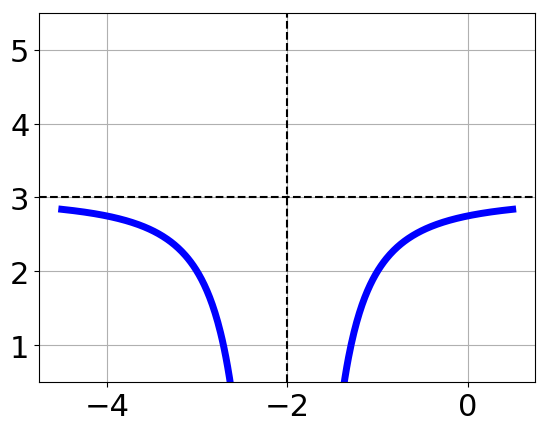
\includegraphics[width = 0.3\textwidth]{../Figures/rationalEquationToGraphAB.png}\item 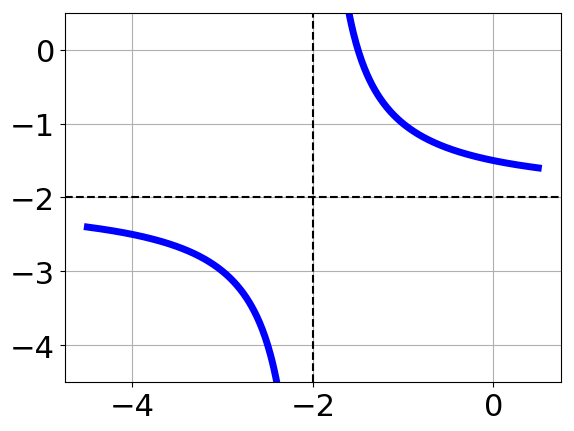
\includegraphics[width = 0.3\textwidth]{../Figures/rationalEquationToGraphBB.png}\item 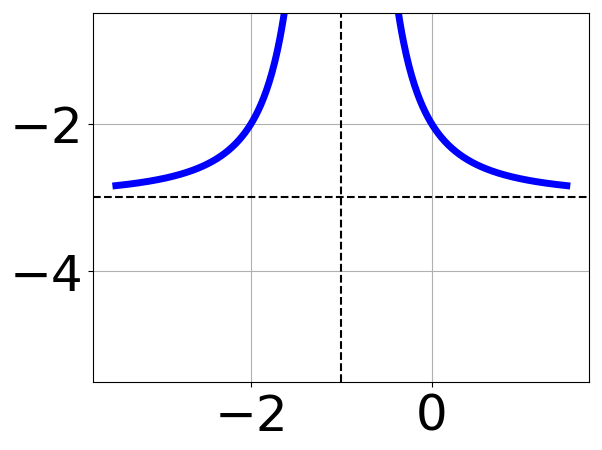
\includegraphics[width = 0.3\textwidth]{../Figures/rationalEquationToGraphCB.png}\item 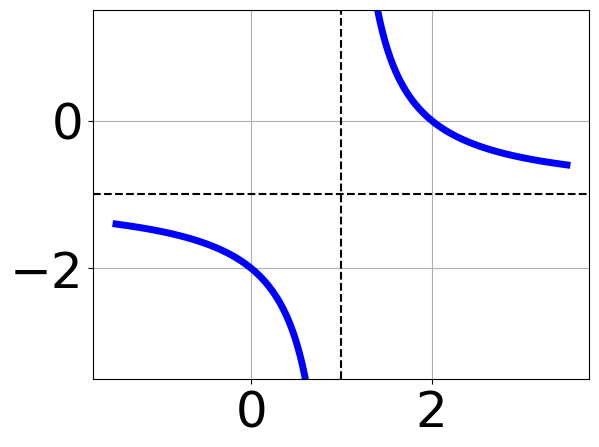
\includegraphics[width = 0.3\textwidth]{../Figures/rationalEquationToGraphDB.png}\end{multicols}\item None of the above.
\end{enumerate} }
\litem{
Choose the equation of the function graphed below.
\begin{center}
    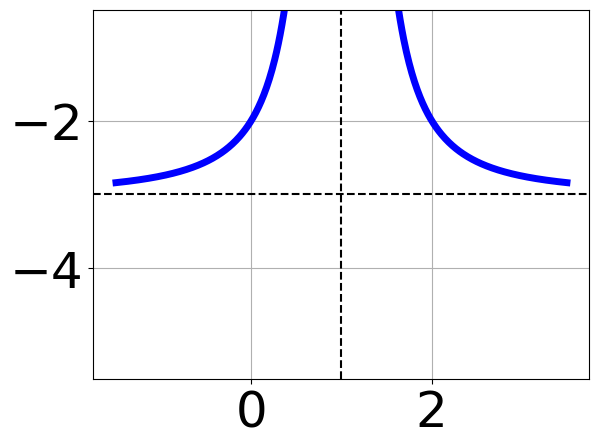
\includegraphics[width=0.5\textwidth]{../Figures/rationalGraphToEquationB.png}
\end{center}
\begin{enumerate}[label=\Alph*.]
\item \( f(x) = \frac{-1}{(x + 1)^2} + 1 \)
\item \( f(x) = \frac{-1}{x + 1} + 1 \)
\item \( f(x) = \frac{1}{x - 1} + 1 \)
\item \( f(x) = \frac{1}{(x - 1)^2} + 1 \)
\item \( \text{None of the above} \)

\end{enumerate} }
\litem{
Solve the rational equation below. Then, choose the interval(s) that the solution(s) belongs to.\[ \frac{9}{-5x + 2} + -6 = \frac{3}{15x -6} \]\begin{enumerate}[label=\Alph*.]
\item \( x_1 \in [-1.1, -0.7] \text{ and } x_2 \in [0,0.14] \)
\item \( \text{All solutions lead to invalid or complex values in the equation.} \)
\item \( x \in [-1.1,-0.7] \)
\item \( x_1 \in [-0.2, 0.4] \text{ and } x_2 \in [0.14,0.48] \)
\item \( x \in [0.07,1.07] \)

\end{enumerate} }
\litem{
Determine the domain of the function below.\[ f(x) = \frac{4}{15x^{2} +27 x + 12} \]\begin{enumerate}[label=\Alph*.]
\item \( \text{All Real numbers except } x = a, \text{ where } a \in [-1.37, -0.98] \)
\item \( \text{All Real numbers except } x = a \text{ and } x = b, \text{ where } a \in [-1.37, -0.98] \text{ and } b \in [-0.84, -0.59] \)
\item \( \text{All Real numbers except } x = a, \text{ where } a \in [-20.28, -19.69] \)
\item \( \text{All Real numbers.} \)
\item \( \text{All Real numbers except } x = a \text{ and } x = b, \text{ where } a \in [-20.28, -19.69] \text{ and } b \in [-9.15, -8.94] \)

\end{enumerate} }
\litem{
Solve the rational equation below. Then, choose the interval(s) that the solution(s) belongs to.\[ \frac{4x}{-4x + 4} + \frac{-5x^{2}}{8x^{2} +4 x -12} = \frac{-6}{-2x -3} \]\begin{enumerate}[label=\Alph*.]
\item \( x_1 \in [0.3, 1.3] \text{ and } x_2 \in [-7.33,-2.33] \)
\item \( x \in [-6.5,-2.7] \)
\item \( x_1 \in [0.3, 1.3] \text{ and } x_2 \in [-2,2] \)
\item \( \text{All solutions lead to invalid or complex values in the equation.} \)
\item \( x \in [-1.8,-0.7] \)

\end{enumerate} }
\litem{
Choose the equation of the function graphed below.
\begin{center}
    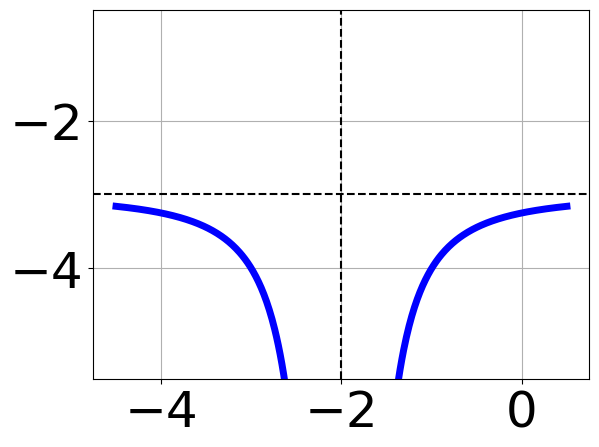
\includegraphics[width=0.5\textwidth]{../Figures/rationalGraphToEquationCopyB.png}
\end{center}
\begin{enumerate}[label=\Alph*.]
\item \( f(x) = \frac{1}{x + 2} - 4 \)
\item \( f(x) = \frac{1}{(x + 2)^2} - 4 \)
\item \( f(x) = \frac{-1}{(x - 2)^2} - 4 \)
\item \( f(x) = \frac{-1}{x - 2} - 4 \)
\item \( \text{None of the above} \)

\end{enumerate} }
\litem{
Choose the graph of the equation below.\[ f(x) = \frac{-1}{(x + 1)^2} - 2 \]\begin{enumerate}[label=\Alph*.]
\begin{multicols}{2}\item 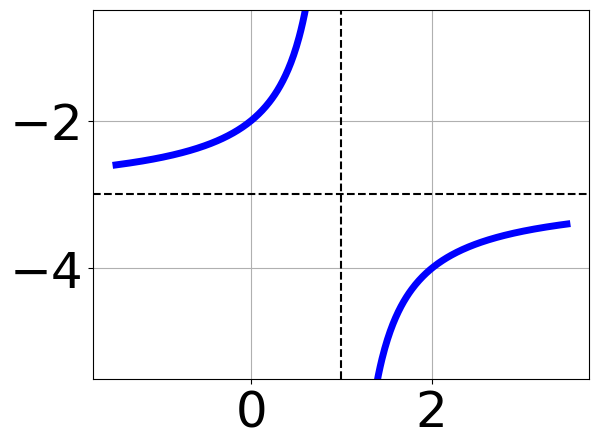
\includegraphics[width = 0.3\textwidth]{../Figures/rationalEquationToGraphCopyAB.png}\item 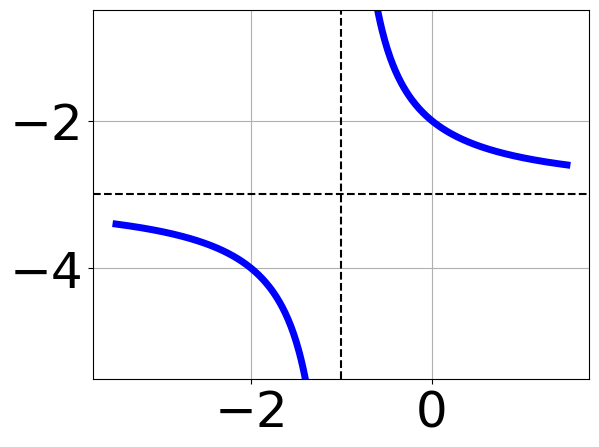
\includegraphics[width = 0.3\textwidth]{../Figures/rationalEquationToGraphCopyBB.png}\item 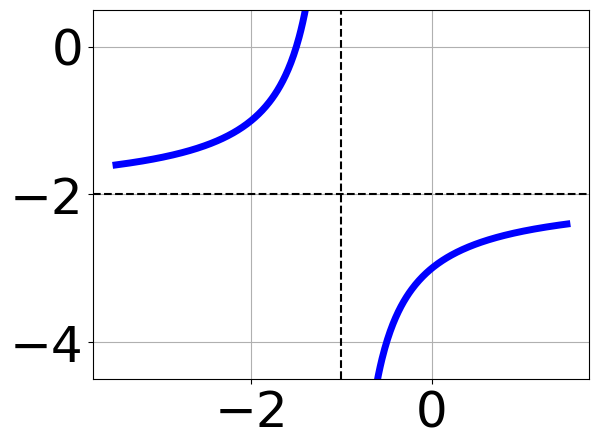
\includegraphics[width = 0.3\textwidth]{../Figures/rationalEquationToGraphCopyCB.png}\item 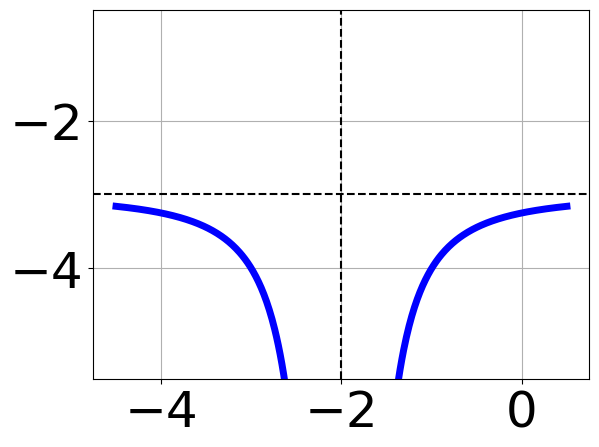
\includegraphics[width = 0.3\textwidth]{../Figures/rationalEquationToGraphCopyDB.png}\end{multicols}\item None of the above.
\end{enumerate} }
\litem{
Solve the rational equation below. Then, choose the interval(s) that the solution(s) belongs to.\[ \frac{39}{117x -91} + 1 = \frac{39}{117x -91} \]\begin{enumerate}[label=\Alph*.]
\item \( x_1 \in [-1, 0.2] \text{ and } x_2 \in [-1.22,1.78] \)
\item \( x \in [0.78,2.78] \)
\item \( x \in [-1,0.2] \)
\item \( x_1 \in [0.5, 1.3] \text{ and } x_2 \in [-1.22,1.78] \)
\item \( \text{All solutions lead to invalid or complex values in the equation.} \)

\end{enumerate} }
\litem{
Solve the rational equation below. Then, choose the interval(s) that the solution(s) belongs to.\[ \frac{3x}{-2x + 2} + \frac{-3x^{2}}{-12x^{2} +6 x + 6} = \frac{4}{6x + 3} \]\begin{enumerate}[label=\Alph*.]
\item \( x \in [-0.62,-0.24] \)
\item \( \text{All solutions lead to invalid or complex values in the equation.} \)
\item \( x \in [-2.46,-1.41] \)
\item \( x_1 \in [-0.35, 1.15] \text{ and } x_2 \in [0.8,1.4] \)
\item \( x_1 \in [-0.35, 1.15] \text{ and } x_2 \in [-4,-1.4] \)

\end{enumerate} }
\litem{
Determine the domain of the function below.\[ f(x) = \frac{5}{20x^{2} +46 x + 24} \]\begin{enumerate}[label=\Alph*.]
\item \( \text{All Real numbers except } x = a \text{ and } x = b, \text{ where } a \in [-1.75, -1.39] \text{ and } b \in [-1.03, -0.71] \)
\item \( \text{All Real numbers except } x = a, \text{ where } a \in [-1.75, -1.39] \)
\item \( \text{All Real numbers except } x = a \text{ and } x = b, \text{ where } a \in [-24.7, -23.67] \text{ and } b \in [-20.31, -19.93] \)
\item \( \text{All Real numbers except } x = a, \text{ where } a \in [-24.7, -23.67] \)
\item \( \text{All Real numbers.} \)

\end{enumerate} }
\end{enumerate}

\end{document}